\chapter{Développement du système de notification Telegram}

\section{Introduction}

Après le développement et la validation du moteur de détection SSH présenté dans le chapitre précédent, l'étape suivante du projet Automated Network Self-Defense System (ANSDS) consiste à informer automatiquement l'administrateur dès qu'un comportement suspect est détecté sur le réseau.

La simple détection d'une attaque ne constitue pas une réponse suffisante face aux menaces actuelles. Un système de sécurité efficace doit être capable de transmettre rapidement les informations relatives à l'incident afin de réduire le temps de réaction de l'administrateur. Cette capacité représente une étape essentielle avant la mise en œuvre de mécanismes de réponse automatique tels que le blocage dynamique d'une adresse IP malveillante.

Dans ce projet, le service de messagerie Telegram a été retenu comme solution de notification. Telegram met à disposition une interface de programmation (Telegram Bot API) permettant à une application d'envoyer automatiquement des messages vers une conversation privée ou un groupe de discussion. Cette API est simple à intégrer dans une application Python et offre un moyen fiable de transmettre des alertes en temps réel.

Afin de conserver une architecture logicielle modulaire, le système de notification a été développé sous la forme d'un composant indépendant du moteur de détection. Cette approche facilite la maintenance du projet, améliore la réutilisabilité du code et prépare l'intégration du futur module de réponse automatique basé sur Netmiko.

Le développement du système de notification a été réalisé de manière progressive. Chaque fonctionnalité a été implémentée puis validée individuellement avant son intégration au moteur de détection développé avec Scapy. Cette méthode garantit la fiabilité de chaque composant et limite les risques d'erreur lors de l'évolution du système.

Dans ce chapitre, nous présentons successivement les objectifs poursuivis, le fonctionnement de Telegram Bot API, la création du bot, le développement du module Python de notification, son intégration avec le moteur de détection SSH, les validations expérimentales réalisées ainsi que les résultats obtenus.

\section{Objectifs de la phase}

Cette phase constitue la première étape du développement du mécanisme de réponse du projet ANSDS.

Les objectifs principaux sont les suivants :

\begin{itemize}

\item créer un bot Telegram destiné à recevoir les alertes de sécurité ;

\item récupérer les informations d'authentification nécessaires à l'utilisation de Telegram Bot API ;

\item développer un module Python réutilisable permettant d'envoyer automatiquement des notifications ;

\item intégrer ce module au moteur de détection SSH développé avec Scapy ;

\item construire un message d'alerte contenant les informations essentielles relatives à l'attaque détectée ;

\item transmettre automatiquement une notification dès que le seuil de détection est atteint ;

\item concevoir une architecture modulaire compatible avec le futur module de réponse automatique basé sur Netmiko ;

\item valider expérimentalement le bon fonctionnement de chaque fonctionnalité développée.

\end{itemize}

À l'issue de cette phase, le système est capable de transmettre automatiquement une notification détaillée à l'administrateur dès qu'une attaque SSH est détectée. Cette fonctionnalité constitue une étape essentielle dans la construction d'un système complet d'auto-défense réseau, puisqu'elle établit le lien entre le moteur de détection et les futurs mécanismes de réponse automatique.

\section{Présentation de Telegram Bot API}

Telegram est une plateforme de messagerie instantanée proposant une interface de programmation appelée Telegram Bot API. Cette interface permet à des applications externes d'interagir automatiquement avec le service Telegram sans intervention humaine.

Le principe repose sur la création d'un bot, c'est-à-dire un compte spécial administré par une application. Contrairement à un utilisateur classique, un bot peut recevoir des commandes, envoyer des messages, transmettre des fichiers et communiquer automatiquement avec les utilisateurs autorisés.

L'accès à Telegram Bot API repose sur un jeton d'authentification (\textit{Bot Token}) généré lors de la création du bot. Ce jeton identifie de manière unique l'application et autorise l'envoi de requêtes vers les serveurs Telegram.

Chaque conversation Telegram possède également un identifiant numérique (\textit{Chat ID}) permettant de spécifier précisément le destinataire des notifications. L'association du Bot Token et du Chat ID permet ainsi au système de transmettre automatiquement les alertes de sécurité à l'administrateur.

Dans le cadre du projet ANSDS, Telegram est utilisé exclusivement comme canal de notification. Toutes les informations produites par le moteur de détection sont transmises au bot afin d'informer immédiatement l'administrateur d'une activité suspecte observée sur le réseau.

\section{Création du Bot Telegram}

La première étape du développement consiste à créer un bot Telegram dédié aux notifications de sécurité.

Telegram met à disposition un service officiel nommé BotFather permettant de créer et d'administrer les bots. Après avoir lancé la commande \texttt{/newbot}, l'utilisateur choisit un nom d'affichage ainsi qu'un nom d'utilisateur unique se terminant obligatoirement par le suffixe \texttt{bot}.

Une fois la création terminée, BotFather génère automatiquement le Bot Token nécessaire à l'authentification auprès de Telegram Bot API.

La Figure~\ref{fig:telegram_bot_creation} présente la création du bot utilisé dans le cadre de ce projet.

\begin{figure}[H]
\centering
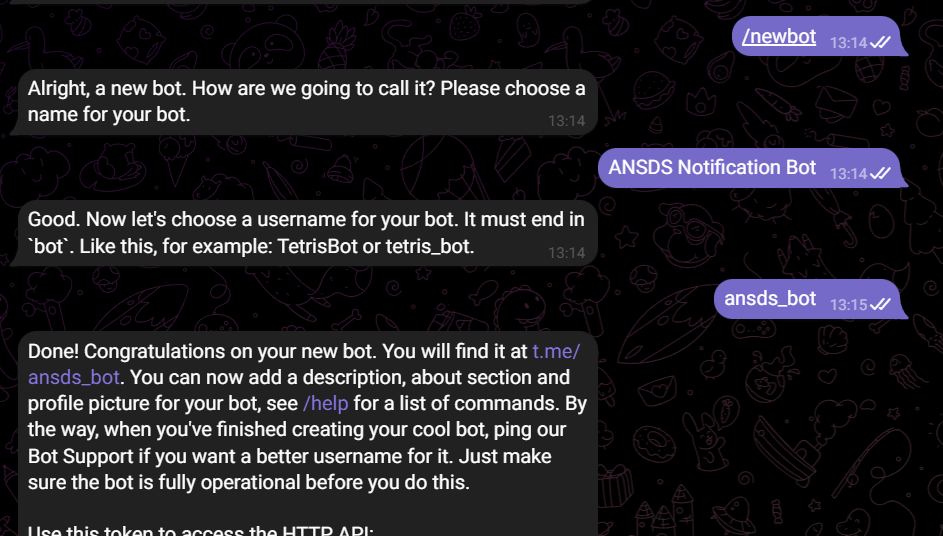
\includegraphics[width=0.92\textwidth]{figures/Fig-03-08_Telegram_Bot_Creation.png}
\caption{Création du bot Telegram avec BotFather}
\label{fig:telegram_bot_creation}
\end{figure}

Le Bot Token constitue une information sensible puisqu'il permet d'accéder au bot et d'envoyer des messages en son nom. Il doit donc être conservé de manière confidentielle et ne jamais être diffusé dans un dépôt Git public.

Après la création du bot, une première conversation privée est ouverte avec celui-ci à l'aide de la commande \texttt{/start}. Cette étape permet à Telegram d'associer un identifiant de conversation (\textit{Chat ID}) au futur destinataire des notifications.

Le Chat ID est ensuite récupéré à l'aide de la méthode \texttt{getUpdates} proposée par Telegram Bot API.

La Figure~\ref{fig:telegram_chat_id} présente la récupération de cet identifiant.

\begin{figure}[H]
\centering
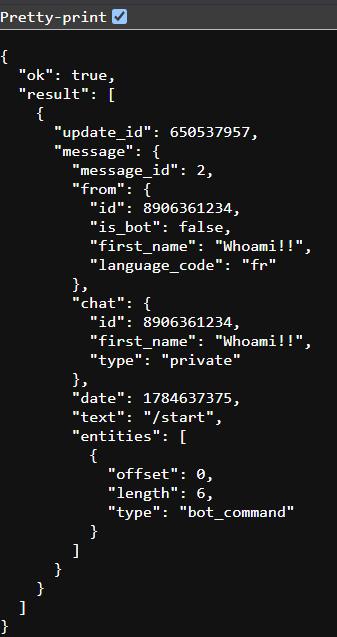
\includegraphics[width=0.92\textwidth]{figures/Fig-03-09_Telegram_Chat_ID.png}
\caption{Récupération du Chat ID}
\label{fig:telegram_chat_id}
\end{figure}

À l'issue de cette première étape, toutes les informations nécessaires à la communication avec Telegram Bot API sont disponibles. Le développement du module Python de notification peut alors commencer.

\section{Développement du module de notification}

Une fois les paramètres d'authentification obtenus, l'étape suivante consiste à développer un module Python capable de communiquer avec Telegram Bot API.

Plutôt que d'intégrer directement les appels HTTP à l'intérieur du moteur de détection, un composant indépendant nommé \texttt{telegram\_notifier.py} est développé. Cette séparation des responsabilités permet de rendre le projet plus modulaire et facilite les évolutions futures.

Le module de notification est chargé exclusivement de transmettre les messages vers Telegram. Il ne réalise aucune opération de détection et ne possède aucune connaissance du fonctionnement interne du moteur Scapy. Cette approche respecte le principe de responsabilité unique (\textit{Single Responsibility Principle}) couramment utilisé dans le développement logiciel.

La communication avec Telegram est réalisée à l'aide de la bibliothèque Python \texttt{requests}. Cette bibliothèque simplifie l'envoi de requêtes HTTP vers Telegram Bot API tout en offrant des mécanismes de gestion des erreurs permettant d'améliorer la robustesse du système.

Le module développé expose une unique fonction publique nommée \texttt{send\_notification()}. Cette fonction reçoit le contenu du message à transmettre, construit la requête HTTP puis vérifie la réponse renvoyée par Telegram avant d'indiquer si l'envoi a été réalisé avec succès.

Cette architecture permet à n'importe quel futur composant du projet d'envoyer une notification sans avoir à connaître les détails de communication avec Telegram.

Une première validation est réalisée afin de vérifier le fonctionnement du module indépendamment du moteur de détection.

La Figure~\ref{fig:first_telegram_message} présente la validation du premier message envoyé depuis Python.

\begin{figure}[H]
\centering
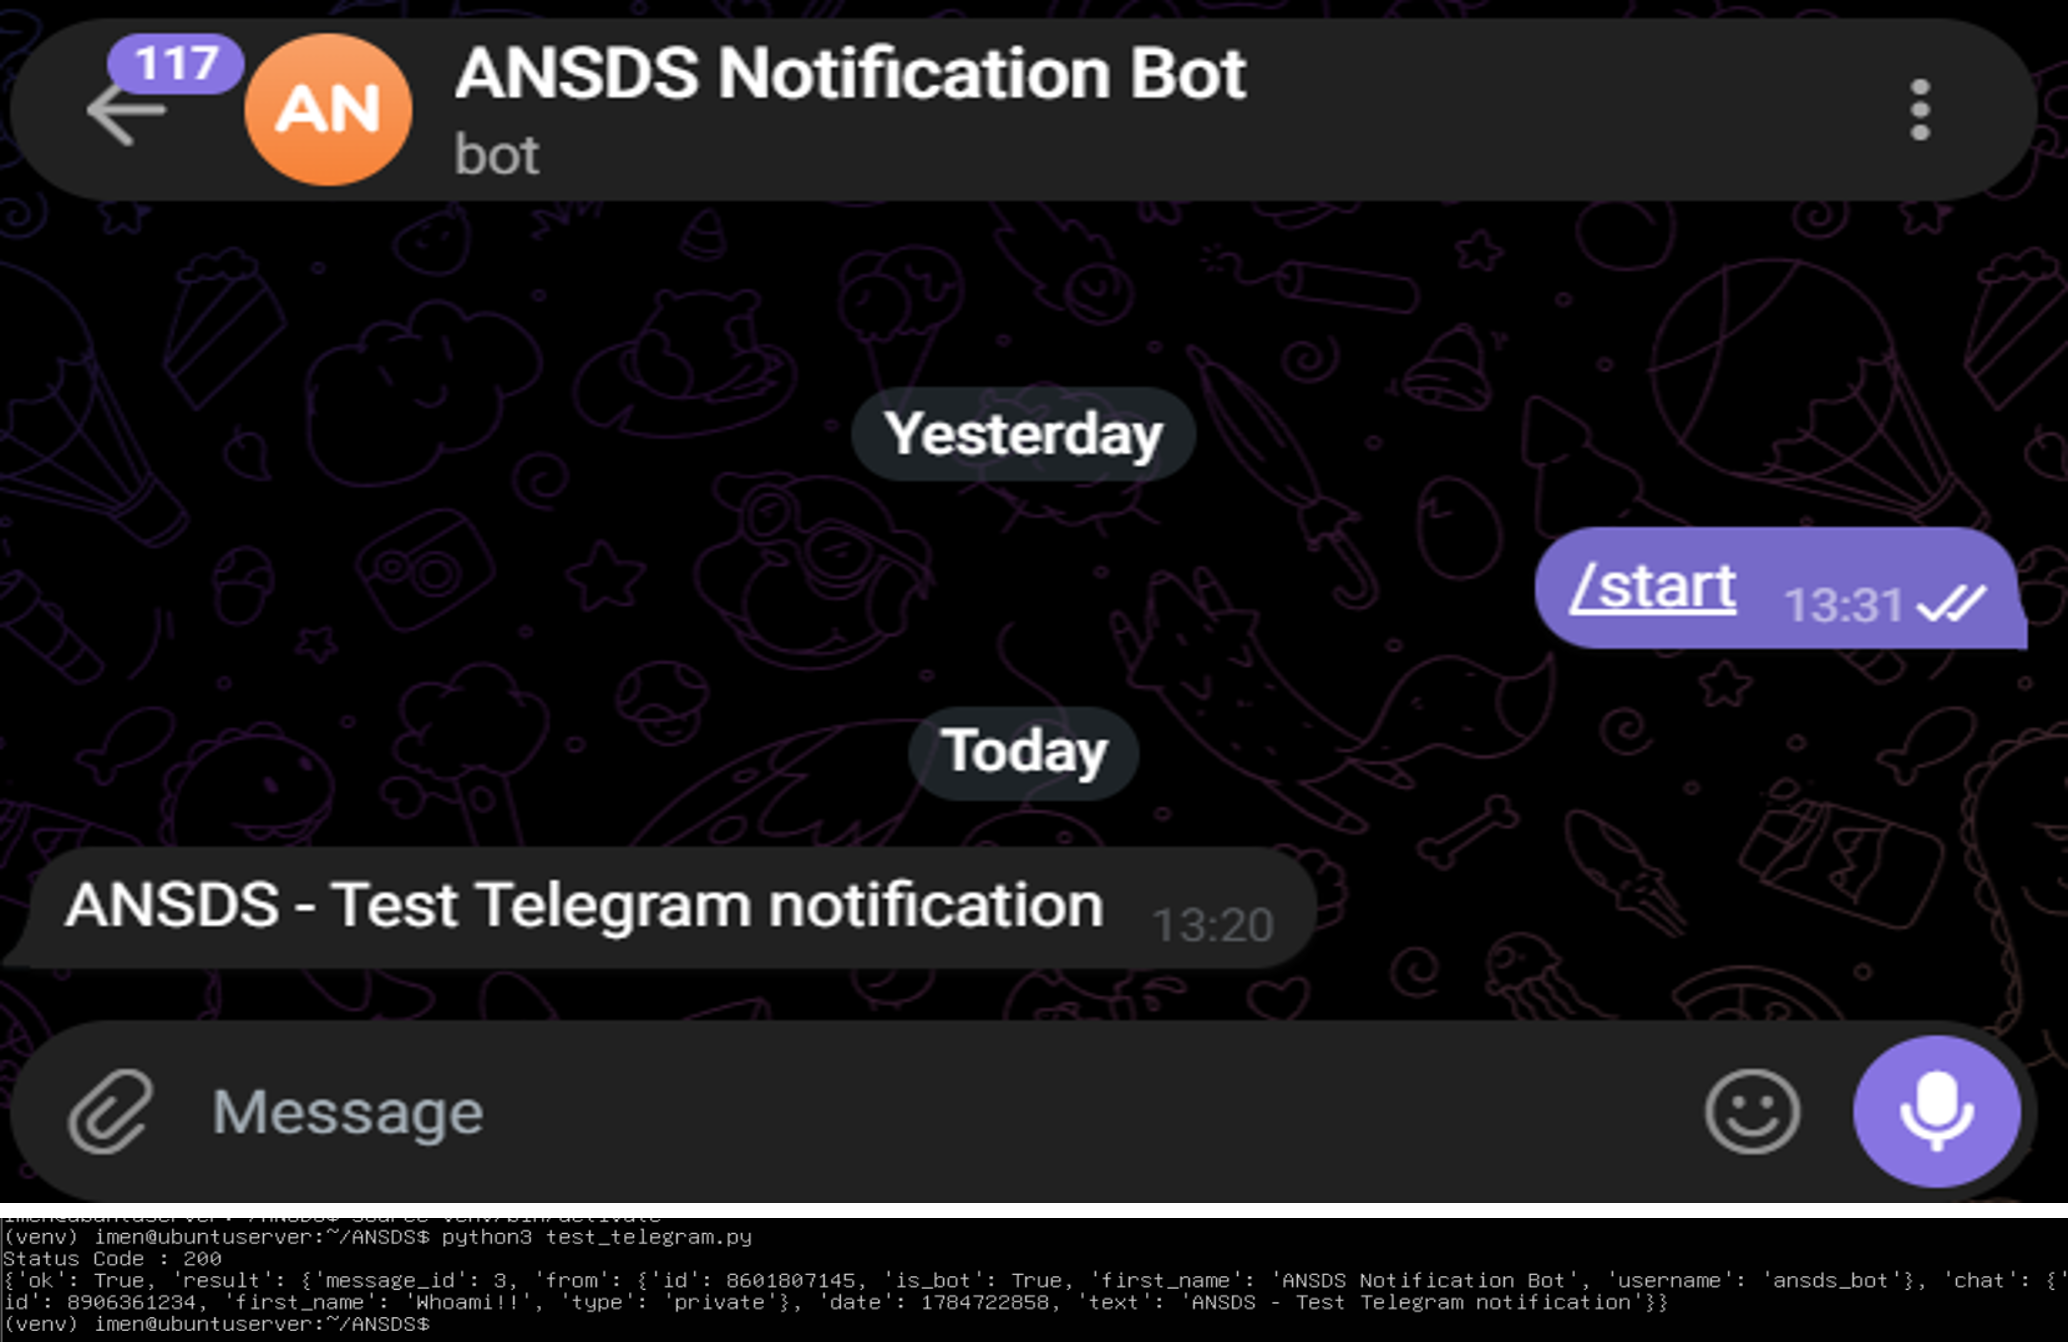
\includegraphics[width=0.92\textwidth]{figures/Fig-03-10_First_Telegram_Test_Message.png}
\caption{Validation du premier message envoyé via Telegram Bot API}
\label{fig:first_telegram_message}
\end{figure}

Après cette première validation, un second script est utilisé afin de vérifier que toutes les communications passent désormais exclusivement par le module \texttt{telegram\_notifier.py}.

Cette étape confirme que la logique de communication est entièrement centralisée dans un composant unique, facilitant ainsi la maintenance du projet.

La Figure~\ref{fig:telegram_module_validation} présente cette validation.

\begin{figure}[H]
\centering
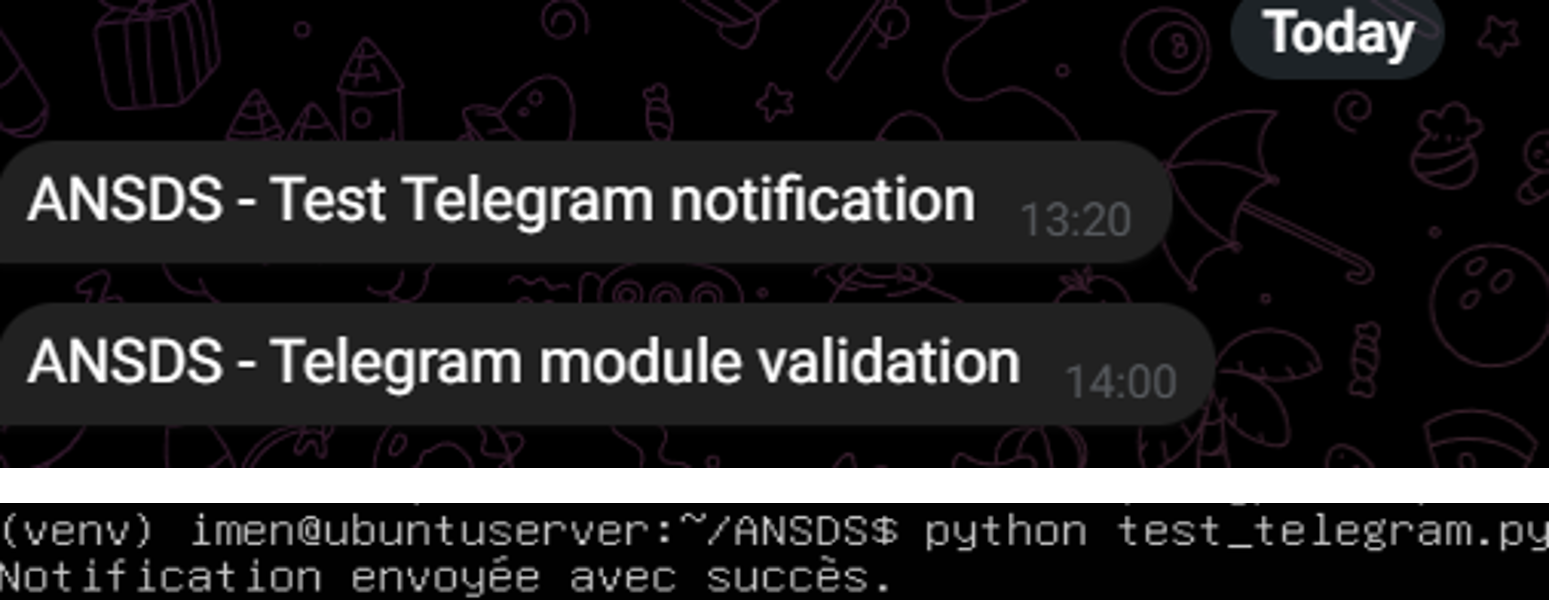
\includegraphics[width=0.92\textwidth]{figures/Fig-03-11_Telegram_Module_Validation.png}
\caption{Validation du module Python de notification}
\label{fig:telegram_module_validation}
\end{figure}

\section{Intégration avec le moteur de détection SSH}

Après la validation indépendante du module de notification, celui-ci est intégré au moteur de détection développé avec Scapy.

L'objectif consiste à automatiser entièrement l'envoi des alertes. Désormais, aucune intervention humaine n'est nécessaire entre la détection d'une attaque et la transmission de la notification.

Le moteur de détection continue d'assurer uniquement l'observation du trafic réseau, le comptage des tentatives de connexion et l'identification des comportements suspects. Lorsqu'une adresse IP dépasse le seuil configuré dans la fenêtre temporelle glissante, le détecteur appelle simplement la fonction \texttt{send\_notification()}.

Cette approche présente plusieurs avantages. Le moteur de détection reste indépendant de Telegram, tandis que le module de notification peut évoluer sans modifier les algorithmes de détection.

Afin d'éviter la génération de notifications multiples lors d'une même attaque, le déclenchement de l'alerte est effectué uniquement lorsque le compteur atteint exactement le seuil configuré. Cette amélioration empêche l'envoi de messages répétitifs tout en garantissant qu'une seule notification est produite pour chaque nouvelle attaque détectée.

L'intégration du module est ensuite validée en générant plusieurs tentatives de connexion SSH depuis la machine Kali Linux.

Le détecteur identifie correctement les paquets TCP SYN, incrémente le compteur associé à l'adresse IP source puis déclenche automatiquement l'envoi d'une notification lorsque le seuil est atteint.

La Figure~\ref{fig:ssh_notification_integration} présente le fonctionnement complet de cette intégration.

\begin{figure}[H]
\centering
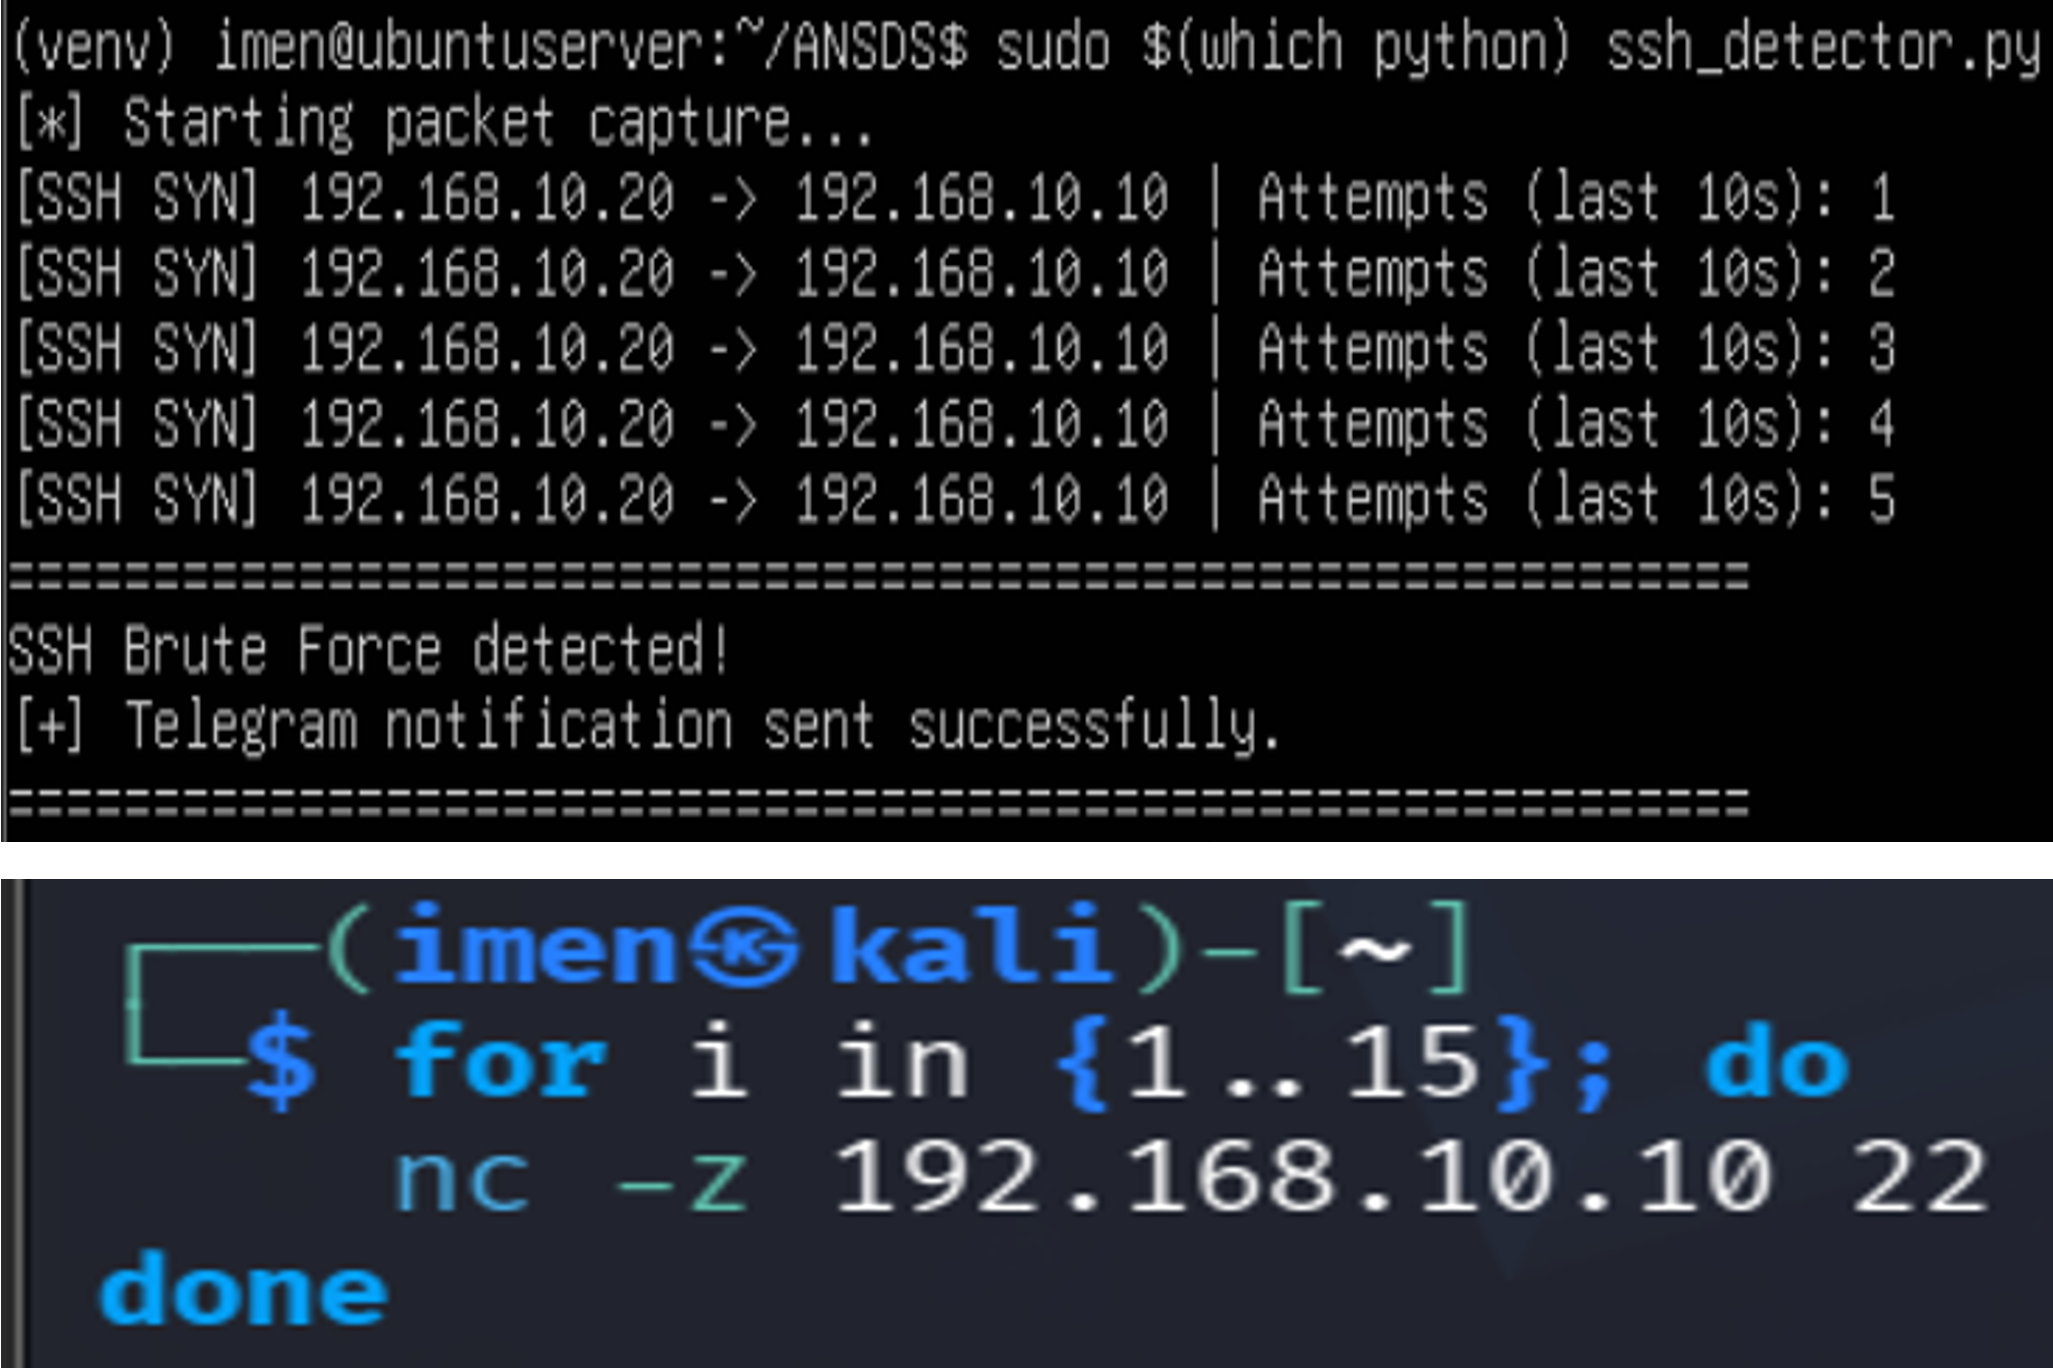
\includegraphics[width=0.92\textwidth]{figures/Fig-03-12_SSH_Detection_With_Telegram_Notification.png}
\caption{Intégration du module Telegram au moteur de détection SSH}
\label{fig:ssh_notification_integration}
\end{figure}

\section{Construction d'une alerte professionnelle}

La première version du système de notification envoyait uniquement un message générique indiquant qu'une attaque SSH avait été détectée.

Bien que cette approche permette de vérifier le bon fonctionnement de Telegram, elle ne fournit pas suffisamment d'informations pour permettre une analyse rapide de l'incident ou une automatisation des actions de réponse.

Le contenu de la notification a donc été enrichi afin de transmettre directement toutes les informations nécessaires à l'administrateur réseau.

Chaque notification contient désormais le type d'attaque détectée, le niveau de gravité, la date et l'heure de détection, les adresses IP source et destination, le port cible, le protocole utilisé, le nombre de tentatives observées ainsi que la durée de la fenêtre temporelle utilisée par le moteur de détection.

Cette structure présente également un intérêt majeur pour la suite du projet. Les informations générées par le moteur de détection pourront être directement réutilisées par le futur module Netmiko afin de construire automatiquement les règles ACL destinées à bloquer l'adresse IP malveillante sur le routeur Cisco.

La Figure~\ref{fig:professional_alert} présente le format final de la notification générée automatiquement par le système.

\begin{figure}[H]
\centering
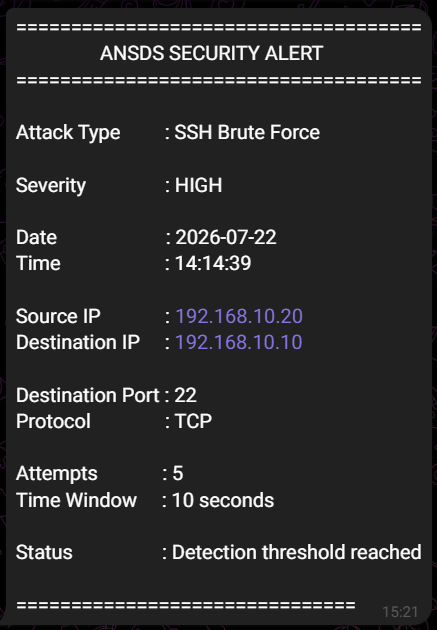
\includegraphics[width=0.92\textwidth]{figures/Fig-03-13_Professional_Telegram_Alert.png}
\caption{Notification de sécurité générée automatiquement par l'ANSDS}
\label{fig:professional_alert}
\end{figure}

\section{Validation expérimentale}

Une série de tests a été réalisée afin de vérifier le bon fonctionnement du système de notification développé durant cette phase. Chaque fonctionnalité a été validée individuellement avant son intégration complète au moteur de détection SSH.

La première validation a consisté à vérifier la création du bot Telegram ainsi que l'obtention des paramètres nécessaires à la communication avec Telegram Bot API. Le Bot Token et le Chat ID ont été récupérés avec succès, permettant ainsi au programme Python de communiquer avec les serveurs Telegram.

Une seconde série de tests a permis de vérifier le fonctionnement du module \texttt{telegram\_notifier.py}. Plusieurs messages de test ont été transmis afin de confirmer la capacité du module à envoyer automatiquement des notifications sans intervention de l'utilisateur.

Après cette validation indépendante, le module de notification a été intégré au moteur de détection développé avec Scapy. Des scénarios simulant une attaque SSH ont ensuite été exécutés depuis la machine Kali Linux.

À chaque tentative de connexion, le détecteur capture les paquets TCP SYN, met à jour le compteur associé à l'adresse IP source puis compare le nombre de tentatives au seuil configuré.

Lorsque le seuil est atteint à l'intérieur de la fenêtre temporelle glissante, une unique notification est automatiquement générée et transmise à l'administrateur via Telegram.

Les différents essais réalisés confirment le bon fonctionnement de l'ensemble de la chaîne de traitement. Les notifications sont envoyées uniquement lorsqu'une activité réellement suspecte est détectée, évitant ainsi la génération d'alertes inutiles.

\section{Analyse des résultats}

Les expérimentations réalisées démontrent que l'intégration de Telegram Bot API constitue une solution simple, fiable et efficace pour assurer la notification automatique des incidents de sécurité.

La séparation entre le moteur de détection et le module de notification améliore considérablement l'architecture logicielle du projet. Chaque composant possède désormais une responsabilité clairement définie, ce qui facilite la maintenance et limite les dépendances entre les différents modules.

Le développement d'un module Python dédié permet également de centraliser l'ensemble des communications avec Telegram. Toute évolution future du système de notification pourra ainsi être réalisée sans modifier les algorithmes de détection développés avec Scapy.

L'amélioration apportée au mécanisme de déclenchement des alertes constitue également un résultat important. Le remplacement d'une condition de type \texttt{count >= THRESHOLD} par une comparaison stricte \texttt{count == THRESHOLD} permet d'éviter l'envoi de notifications multiples lors d'une même attaque tout en conservant une excellente réactivité.

L'enrichissement du contenu des notifications représente une étape essentielle dans la construction du système d'auto-défense réseau. Les informations transmises ne servent plus uniquement à informer l'administrateur, mais constituent également les données qui seront exploitées par le futur module de réponse automatique.

Cette conception permet de préparer naturellement l'intégration de Netmiko sans modifier l'architecture existante. Les informations relatives à l'attaque pourront être directement utilisées pour générer dynamiquement les règles de filtrage sur le routeur Cisco.

Les résultats obtenus confirment ainsi la pertinence de l'architecture retenue ainsi que la faisabilité de la chaîne complète de détection et de notification développée au cours de cette phase.

\section{Conclusion}

Cette phase a permis de développer le premier mécanisme de réponse du système Automated Network Self-Defense System.

À partir du moteur de détection SSH développé avec Scapy, le système est désormais capable de transmettre automatiquement une notification détaillée dès qu'un comportement compatible avec une attaque par force brute est identifié.

Les différentes fonctionnalités développées comprennent la création d'un bot Telegram, la communication avec Telegram Bot API, le développement d'un module Python réutilisable, l'intégration de ce module au moteur de détection ainsi que la génération d'une notification professionnelle contenant toutes les informations nécessaires à l'analyse de l'incident.

Les validations expérimentales réalisées démontrent le bon fonctionnement de l'ensemble du sous-système de notification ainsi que la robustesse de son intégration avec le moteur de détection.

Cette nouvelle capacité constitue une étape majeure dans la construction de l'Automated Network Self-Defense System. Le système ne se limite désormais plus à détecter une activité suspecte, mais devient capable d'informer automatiquement l'administrateur en temps réel.

La phase suivante sera consacrée au développement du module de réponse automatique basé sur Netmiko. Celui-ci exploitera directement les informations générées par le moteur de détection et le système de notification afin de configurer automatiquement des listes de contrôle d'accès (ACL) sur le routeur Cisco et d'isoler dynamiquement les adresses IP malveillantes.